% Set up the document
\documentclass{article}

% Page size
\usepackage[
    letterpaper,]{geometry}

% Lines between paragraphs
\setlength{\parskip}{\baselineskip}
\setlength{\parindent}{0pt}

% Math
\usepackage{mathtools}
\usepackage{amssymb}
\usepackage{commath}

% Math notation macros
\def\*#1{\mathbf{#1}}
\newcommand{\dadvd}[2]{\dfrac{\text{D} #1}{\text{D} #2}} % advective derivative

\newcommand{\fS}{\mathcal{S}} % fancy S

\newcommand{\nhat}{\mathbf{\hat{n}}}
\newcommand{\rhat}{\mathbf{\hat{r}}}
\newcommand{\thetahat}{\boldsymbol{\hat{\theta}}}
\newcommand{\xhat}{\mathbf{\hat{x}}}
\newcommand{\yhat}{\mathbf{\hat{y}}}
\newcommand{\zhat}{\mathbf{\hat{z}}}
\newcommand{\omegavec}{\boldsymbol{\omega}}

% Links
\usepackage{hyperref}

% Page numbers at top right
\usepackage{fancyhdr}
\pagestyle{fancy}
\fancyhf{}
\fancyhead[R]{\thepage}
\renewcommand\headrulewidth{0pt}

% Graphics
\usepackage{float}
\usepackage{graphicx}
\graphicspath{ {./img/} }

\begin{document}

\textbf{MATH 462 Assignment 5} \\
\textbf{Matt Wiens \#301294492} \\
\textbf{2020-02-12}

\textbf{A) A Patch of Vorticity.}
Consider an incompressible, but rotational, 2D fluid whose initial
condition is characterized by a circular patch of vorticity
%
\begin{equation*}
    \omega(\*x, 0) =
        \begin{dcases}
            \frac{1}{\pi a^2},& 0 \leq r < a \\
            0,& a < r < \infty
        \end{dcases}
        ,
\end{equation*}
%
where $\omega$ is the $\zhat$-component of vorticity $\omegavec$ and $r
= |\*x|$.

\textbf{i)} Solve for the initial streamfunction $\psi(\*x, 0)$, and
hence determine the initial flow velocity. Your task is simplified in
this geometry since the Poisson PDE for the streamfunction $\psi(\*x,
0)$ is really just an ODE in polar coordinates. Invoke the boundary
values that the flow is bounded at the origin, and decays to zero as $r
\to \infty$. It is also necessary to impose continuity on the
streamfunction and its associated flow at $r = a$. Choose the constant
part of the streamfunction to be zero at $r \to \infty$. Describe the
resulting flow pattern.

\textbf{ii)} Using the vorticity equation, deduce the time evolution of
this flow for $t > 0$. This result, in turn, makes it easy to determine
the pressure field. Invoke the conditions that the pressure approaches a
constant value $p^\infty$ as $r \to \infty$ and is continuous at $r =
a$. Explain why the pressure field is consistent with the flow pattern.

\textbf{iii)} Make a subplot or two showing the important flow
quantities (what should these be?) as a function of $r$.

\textbf{iv)} Finally, show that there is a limiting streamfunction as the patch
parameter $a \to 0$,
%
\begin{equation*}
    \psi_0(\*x, t) = \lim_{a \to 0} \psi(\*x, t)
    .
\end{equation*}
%
Acheson refers to this limit as the line vortex of 3D flow.

\textbf{v)} (This part is optional.) Evaluate two types of circulation
integrals. The first are circular loops centered at the origin with $r =
R$. The second are circular loops that do not enclose (or include) the
origin. One of these evaluations is a calculation; the other is a
mathematical argument.

\newpage

\textbf{Solution}

\newpage

\textbf{B) Circulation as a constant of the Flow.}
The circulation integral was introduced for its connection to the
vorticity via the Stokes theorem,
%
\begin{equation*}
    \Lambda_{\partial \fS}
        = \oint_{\partial \fS (t)} \*u \cdot \dif \*x
        = \iint_{\fS} \del{\nabla \times \*u} \cdot \nhat \dif S
        ,
\end{equation*}
%
where $\partial \fS$ is a simple closed curve within the flow that is a
boundary for the open surface $\fS$. However, when this integral
$\Lambda_{\partial \fS (t)}$ is considered on a curve being advected by
the flow, the idea of circulation is elevated in importance by the
Kelvin circulation theorem. As in the opening of Chapter 5 in Acheson,
the theorem is the conservation principle
%
\begin{equation*}
    \dod{}{t} \Lambda_{\partial \fS (t)} = 0
    .
\end{equation*}
%
The justification is contained in the chapter (partially as Problem
5.2), but you are being asked to derive this result using a mathematical
difference quotient approach, with proper limits being stated. Follow
the outline and the cartoon sketch below.
%
\begin{figure}[!ht]
    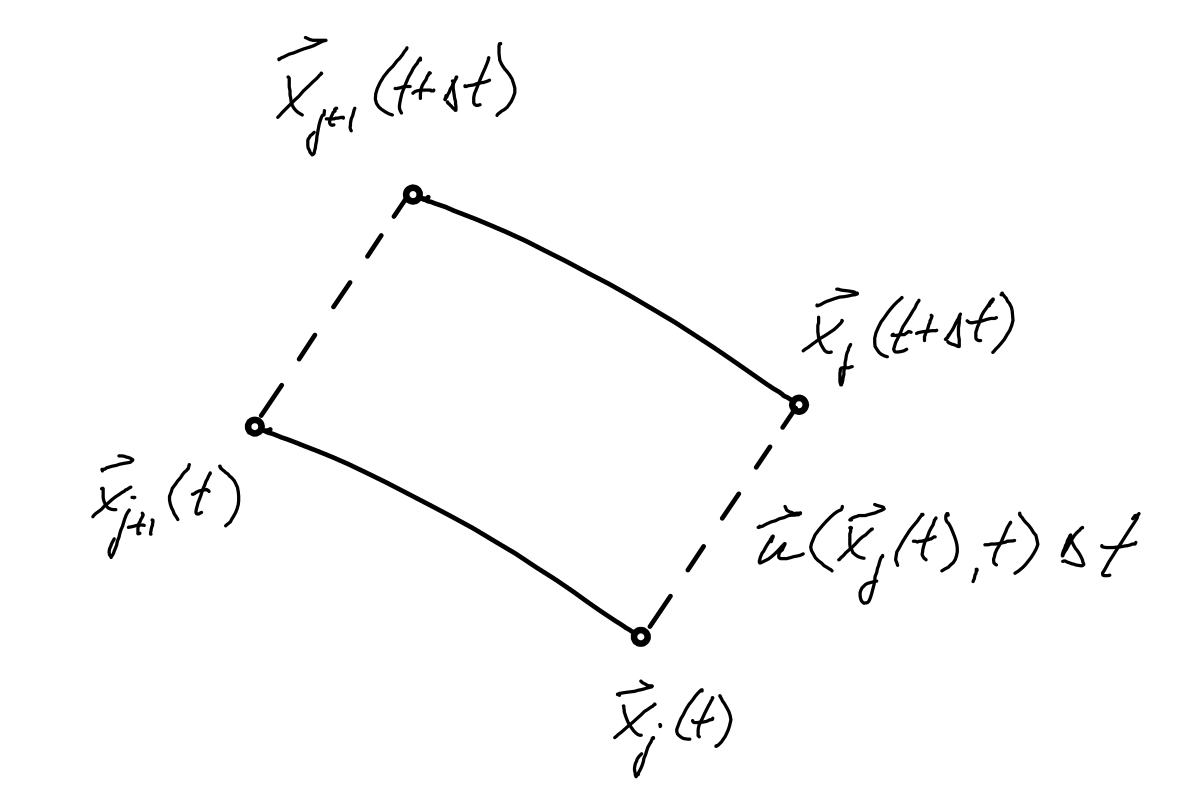
\includegraphics[width=14em]{b-diag}
    \centering
\end{figure}

1) Express the integral
%
\begin{equation*}
    \Lambda_{\partial \fS (t)} = \oint_{\partial \fS} \*u(\*x, t) \cdot \dif \*x
\end{equation*}
%
as a Riemann sum over the intervals $\Delta \*x_j = \*x(t)_{j + 1} -
\*x(t)_j$ where $|\Delta \*x_j| \to 0$ gives the limit to the integral.
But what value should you use for the $\*u$? It really doesn't matter,
but the most robust choice for many will be the trapezoidal rule that
takes the average between the values at $\*x(t)_j$ and $\*x(t)_{j + 1}$.

2) Now write the Riemann sum for the circulation integral at $t + \Delta
t$, and form the difference quotient for the $t$-derivative.

3) The difference quotient expression can be broken up into two sums,
only one of which immediately has the form of a Riemann sum. Evaluating
the limits associated with this Riemann sum results in the derivation as
sketched out in Acheson.

4) But what about the other sum? This is where the midpoint rule works
its magic---it forms a telescoping sum. And since the integral is
over a closed loop, the net contribution is zero!

\newpage

\textbf{Solution}

\end{document}
